\documentclass[journal]{IEEEtran}
%\usepackage{cite}
\usepackage{graphicx}
%\usepackage{circuitikz}
%\usepackage[cmex10]{amsmath}
%\usepackage{dblfloatfix}
%\usepackage{capt-of}
%\usepackage{breqn}
%\usepackage{listings}
%\usepackage{mathrsfs}
%\usepackage[scale=.8]{geometry}
%\usepackage{hyperref}
%\usepackage{breakurl}
\usepackage{epstopdf}
\usepackage[nomarkers,nolists,tablesfirst]{endfloat}
\renewcommand{\efloatseparator}{\mbox{}}

\begin{document}
% paper title
% can use linebreaks \\ within to get better formatting as desired
\title{A Switched-Capacitor Amplifier for Use in a 2.5bit/stage Pipelined Analog-to-Digital Converter }

\author{Joseph Meyer and Miles Sherman}

% The paper headers
\markboth{ELEN 6312 Advanced Analog Integrated Circuits}%
{Shell \MakeLowercase{\textit{et al.}}: Bare Demo of IEEEtran.cls for Journals}
\maketitle

\begin{abstract}
A switched-capacitor amplifier with a nominal gain of 4 was designed for use in a 2.5 bit/stage pipelined analog-to-digital converter (ADC). The total resolution of the ADC was 10 bits. The sample rate of the ADC was $5kS/s$. During the sample phase, differential input voltage was sampled onto 4 capacitors on each differential input. During the hold phase, the stored charge was transfered onto 1 hold capacitor in feedback around an operational transconductance amplifier (OTA). The OTA consisted of a pMOS-input folded cascode stage followed by an nMOS common source stage. The open loop DC gain of the OTA was $110.9dB$. The unity gain bandwidth of the OTA was $87.1kHz$. The circuit consumed $769.5nW$ of DC power. Using DC power, this amplifier achieved a Figure of Merit of $150fJ$ per conversion step.
\end{abstract}

% Note that keywords are not normally used for peerreview papers.
\begin{IEEEkeywords}
switched-capacitor amplifier, pipelined analog-to-digital converter
\end{IEEEkeywords}

\section{Introduction}
\IEEEPARstart {P}{ipelined} ADCs require accurate amplification in each stage for proper operation. The residue of each stage must be amplified to be properly processed by the subsequent stage. Pipelined ADCs implementing 2.5 bits per stage with comparator redundancy require a gain of 4. 

Switched-capacitor amplifiers are ideal for accurate amplifiers. Since the gain of switched-capacitor amplifiers relies only on ratios of capacitors (as opposed to ratios of multiple types component values), the gain of these amplifiers tends to be quite accurate.

\section{System Level Design}
\subsection{Top Level Schematic}
The schematic overall system level design is shown in Figure \ref{fig:system_level_schem}. With ideal switches and ideal OTA, this schematic yields an exact gain of 4. This section overviews the specifications for each of these components.

\begin{figure}
\centering
\includegraphics[width=5in]{Schematics/system_level_schem.png}
\caption{The system level schematic of the switched-capacitor amplifier.}
\label{fig:system_level_schem}
\end{figure}

\subsection{Common Mode Voltage}
We know that the common mode voltage at the input and output nodes should be the same for proper operation of the device. To maximize the voltage swing at the output, we must choose $V_{CM}$ to be exactly at mid-rail. Thus,
\begin{equation}
V_{cm}=\frac{V_{DD}}{2}=0.9V
\end{equation}

\subsection{Full Scale Voltage}
In our design, we can assume that the output of the OTA can swing between $V_{ov}$ and $V_{DD}-V_{ov}$. If we choose our $V_{FS}$ to occupy the entire swing at the output and make the assumption that $V_{ov}\approx 0.2V$, we find that
\begin{equation}
V_{FS} = \left(V_{DD} - V_{ov}\right) - V_{ov} = 1.4V
\end{equation}

\subsection{Least Significant Bit Voltage}
In our differential amplifier topology, the output can swing from $-V_{FS}$ to $V_{FS}$. Thus, we can calculate our least significant bit voltage as
\begin{equation}
V_{LSB}=\frac{2V_{FS}}{2^{10}}=2.73mV
\end{equation}

\subsection{Sample and Hold Capacitors}
We can find the minimum value of the hold and capacitor values from the noise requirements. The specification requires that the noise stored on the capacitors in the circuit be less than half of the quantization noise in the given ADC stage. 

Since this is a differential circuit, each half of the circuit contributes noise to the differential input nodes of the OTA. The noise power of each half circuit adds at these inputs. Since there are four capacitors in parallel during the sample phase, their equivalent capacitance is four times a single sample capacitor. Thus, we can calculate the minimum sample capacitance as
\begin{equation}
C_{samp,min}=\frac{kT}{2\left(\frac{V_{LSB}^2}{24}\right)}=6.65fF
\end{equation}

We found that using sample capacitances in this range provided unacceptable closed loop responses when used in the complete system. In the case of $C_{samp}=15fF$ a full scale input step, output values were approximately $8V_{LSB}$ higher than $V_{FS}$. This result was unacceptable. We found that to have the error at the output be $\approx V_{LSB}$, we required $C_{samp}=150fF$. The various parasitic capacitances throughout the system level design, especially at the inputs to the OTA, were believed to have necessitated the difference between the minimum tolerable capacitance due to noise and the implemented capacitance.

\subsection{Switches}
The implementation of the switches used were complimentary pass transistors, as shown in Figure \ref{fig:switch_schem}. The width and length of the pMOS and nMOS transistors were chosen to be the same such that any injected charge would be canceled. For complimentary pass transistors of equal sizes, the equivalent resistance is given by
\begin{equation}
R_{on} = \frac{1}{\left(\beta_n+\beta_p\right)\left(\frac{W}{L}\right)V_{ov}}
\end{equation}
For minimum sized devices in width and length, $R_{on}=11520\Omega$. Even this value provided a sampling phase time constant that was much faster than required.

\begin{figure}
\centering
\includegraphics[width=2in]{Schematics/switch.eps}
\caption{The schematic of the complimentary pass transistors used as switches at the system level.}
\label{fig:switch_schem}
\end{figure}

\subsection{Clocks}
The clocks used were two non-overlapping clocks, each with a frequency of $5kHz$. The non-overlapping clocks were buffered by a set of the three inverters as shown in Figure \ref{fig:clock_buffer}.

\begin{figure}
\centering
\includegraphics[width=3in]{Schematics/clk_buffer_n.eps}
\caption{The schematic of the complimentary pass transistors used as switches at the system level.}
\label{fig:clock_buffer}
\end{figure}

\subsection{System Level Component Values}
The sizes of the transistors used in the switches and clock buffers are shown in Table \ref{tab:sys_trans_sizes}. The sizes of the sample and hold capacitors are shown in Table \ref{tab:passive_elements}.

\begin{table}
\centering
\caption{System Level Transistor Sizes}
\label{tab:sys_trans_sizes}
\begin{tabular}{|c|c|c|c|}
\hline Transistor & Width (nm) & Length (nm) & Aspect Ratio \\ 
\hline Switch nMOS & 190 & 180 & 1.055 \\ 
\hline Switch pMOS & 190 & 180 & 1.055 \\ 
\hline Clock Buffer nMOS & 1020 & 250 & 4.08 \\
\hline Clock Buffer pMOS & 250 & 250 & 1 \\  
\hline 
\end{tabular} 
\end{table}

\subsection{OTA Parameters}
From our settling requirements, we can find both the required unity gain bandwidth and DC gain for the OTA.

For a full scale step input, the input referred error must be less than $\frac{V_{LSB}}{4}$. This corresponds to an error at the output of $V_{LSB}$. To determine our specifications, we can allocate half of this error to gain error and the other half to settling error.

For the allocated error of $\frac{V_{LSB}}{2}$ due to gain error at the output , the required closed loop DC gain can be found as 
\begin{equation}
A_f = \frac{V_{FS}-\frac{V_{LSB}}{2}}{\frac{V_{FS}}{4}}=3.9961
\end{equation}
This closed loop gain, with $\beta=\frac{1}{4}$, corresponds to an open loop gain of
\begin{equation}
A = \frac{A_f}{1-A_f\beta}=72.2dB
\end{equation}

For the allocated error of $\frac{V_{LSB}}{2}$ due to settling error at the output, the acceptable percentage error can be found as
\begin{equation}
E_{percent}=1-\frac{V_{FS}-\frac{V_{LSB}}{2}}{V_{FS}}=9.7\times 10^{-2}\%
\end{equation}

This corresponds to having settled for $6.9315\tau$. For a sampling rate of $5kS/s$, our required $3dB$ bandwidth of the closed loop system is $11.0kHz$. For $\beta=\frac{1}{4}$, this corresponds to a unity gain bandwidth of $44.1kHz$.

\section{Transistor Level OTA Design}
The transistor level implementation of the OTA is shown in Figure \ref{fig:OTA_schem}.

\begin{figure}
\centering
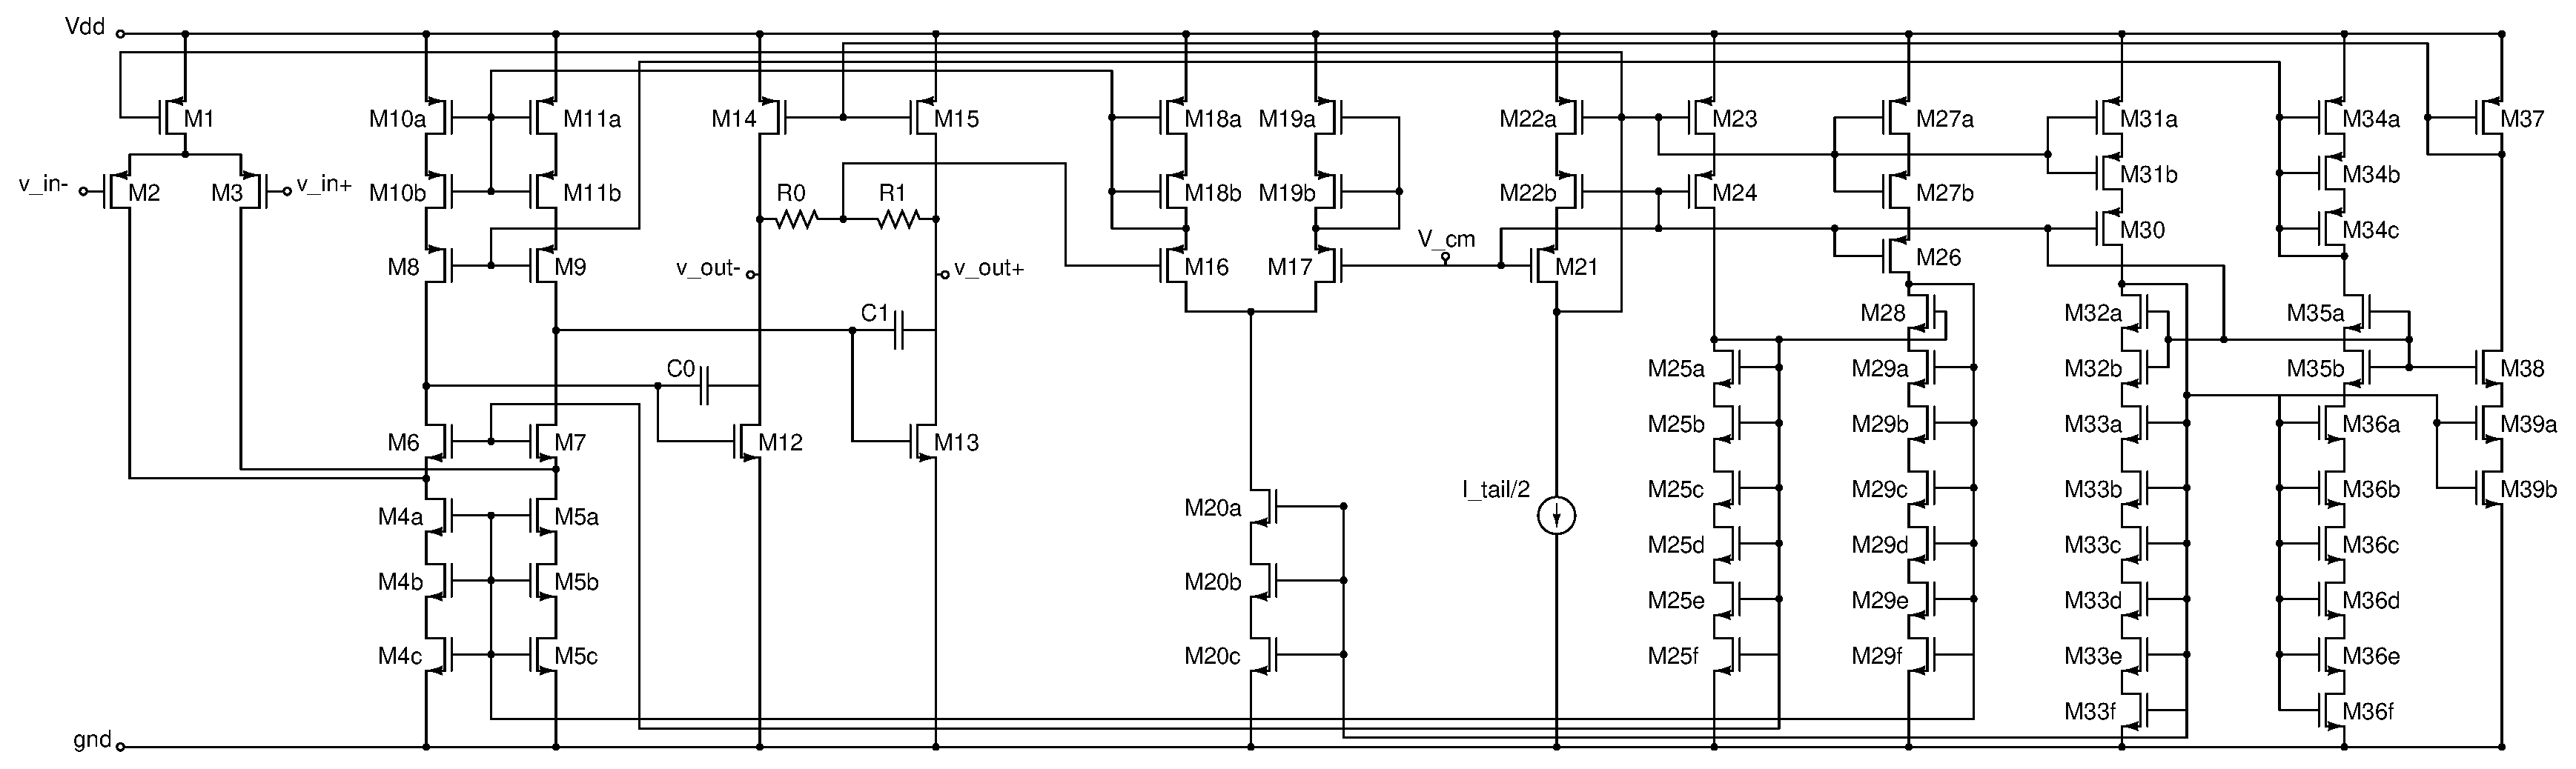
\includegraphics[width=9in,angle=90]{Schematics/OTA.eps}
\caption{The transistor level schematic diagram of the OTA.}
\label{fig:OTA_schem}
\end{figure}

\subsection{Gain Stage}
The OTA implemented a folded-cascode stage followed by a common source stage. This topology was chosen for a number of reasons. First, the required DC gain necessitated an open loop gain on the order of $\approx \left(g_mr_o\right)^3$. Second, an output common source stage allowed for the use of a Miller compensation capacitor. Since the required unity gain bandwidth was small, a Miller compensation capacitor could enable a phase margin well in excess of $60degrees$. Third, an output common source stage allows for more output voltage swing than an output cascode stage.

After choosing a sampling capacitor value $C_{samp}=150fF$, the compensation capacitor was chosen to be $C_{comp}=5C_{samp}=750fF$. To calculate our bias currents in each branch, we first chose that the current in the common source stage was twice the tail current of the folded cascode stage. We can estimate the minimum acceptable bias current of the common source stage as follows. We know that the maximum slew rate our system could encounter will be given by
\begin{equation}
slew_{max} = \frac{2V_{FS}}{\frac{1}{2f_s}}=28k\frac{V}{s}
\end{equation}
since our output can change from one full scale voltage to the other during just one hold phase of the clocks.

Since we can relate the slew rate and the compensation capacitance to the current, we find
\begin{equation}
I_{slew}=I_{bias,cs} = C_{comp}slew_{max}=21nA
\end{equation}

Given this minimum bias current, we chose the bias current of the common source stages to be $70nA$ to ensure settling occurred with the requisite accuracy. This choice yields a folded cascode tail current of $35nA$.

To maximize the amount of DC gain that was achieved for this current, transistors $M2$, $M3$, $M6$, $M7$, $M8$, $M9$, $M12$ and $M13$ were placed into weak inversion; their inversion coefficients were chosen to be $0.1$. Having decreased $f_T$ for these transistors was acceptable since the required unity gain bandwidth of the circuit was so low.

\subsection{Biasing}
The majority of the biasing transistors were biased in moderate-strong inversion. Their inversion coefficients were chosen to be around 2. These included transistors $M1$, $M4$, $M5$, $M10$, $M11$, $M14$, $M15$, $M22$, $M23$, $M25$, $M27$, $M29$, $M31$, $M32$, $M33$, $M34$, $M35$, $M36$, $M39$ and $M37$. To achieve accurate current mirroring through all of the bias branches, transistors such as $M24$, $M28$ and $M32$ were implemented to set matching drain voltages on other bias transistors.

Since many of the transistor lengths calculated were above the maximum transistor length, in many cases transistors were stacked with their gates connected to achieve an equivalent transistor of the appropriate length. Transistors $M25a$ to $M25f$ form a single equivalent $M25$ with  six times the length of one of the transistors in the stack.

\subsection{Component Values}
Table \ref{tab:passive_elements} shows the values of the passive elements used in the OTA. Table \ref{tab:trans_sizes} shows the sizes of the transistors used in the OTA.

\begin{table}
\centering
\caption{Passive Component Values}
\label{tab:passive_elements}
\begin{tabular}{|c|c|}
\hline Component & Value \\ 
\hline Resistors & $\Omega$ \\ 
\hline R0 & 40M \\ 
\hline R1 & 40M \\ 
\hline Capacitors & $fF$ \\ 
\hline $C_{comp}$ & 750 \\ 
\hline $C_{hold}$ & 150 \\ 
\hline $C_{samp}$ & 150 \\ 
\hline 
\end{tabular} 
\end{table}

\begin{table}
\centering
%\caption{OTA Transistor Sizes}
\label{tab:trans_sizes}
\begin{tabular}{|c|c|c|c|}
\hline Transistor & Width (nm) & Length (nm) & Aspect Ratio \\ 
\hline M1 & 300 & 8000 & 0.0375 \\ 
\hline M2 & 750 & 1000 & 0.75 \\ 
\hline M3 & 750 & 1000 & 0.75 \\ 
\hline M4a & 281 & 10000 & 0.0281 \\ 
\hline M4b & 281 & 10000 & 0.0281 \\ 
\hline M4c & 281 & 10000 & 0.0281 \\ 
\hline M5a & 281 & 10000 & 0.0281 \\ 
\hline M5b & 281 & 10000 & 0.0281 \\
\hline M5c & 281 & 10000 & 0.0281  \\
\hline M6 & 250 & 1330 & 0.188 \\
\hline M7 & 250 & 1330 & 0.188 \\
\hline M8 & 750 & 1000 & 0.75 \\
\hline M9 & 750 & 1000 & 0.75 \\
\hline M10a & 281 & 7500 & 0.0375 \\
\hline M10b & 281 & 7500 & 0.0375 \\
\hline M11a & 281 & 7500 & 0.0375  \\
\hline M11b & 281 & 7500 & 0.0375 \\
\hline M12 & 500 & 1000 & 0.5 \\
\hline M13 & 500 & 1000 & 0.5  \\
\hline M14 & 300 & 4000 & 0.075 \\
\hline M15 & 300 & 4000 & 0.075  \\
\hline M16 & 250 & 4000 & 0.0625 \\
\hline M17 & 250 & 4000 & 0.0625  \\
\hline M18a & 250 & 6800 & 0.0368 \\
\hline M18b & 250 & 6800 & 0.0368  \\
\hline M19a & 250 & 6800 & 0.0368 \\
\hline M19b & 250 & 6800 & 0.0368 \\
\hline M20a & 281 & 10000 & 0.0281 \\
\hline M20b & 281 & 10000 & 0.0281  \\
\hline M20c & 281 & 10000 & 0.0281  \\
\hline M21 & 750 & 1000 & 0.75 \\
\hline M22a & 300 & 8000 & 0.0375 \\
\hline M22b & 300 & 8000 & 0.0375 \\
\hline M23 & 300 & 8000 & 0.0375 \\
\hline M24 & 1500 & 1000 & 1.5 \\
\hline M25a & 250 & 10000 & 0.025 \\
\hline M25b & 250 & 10000 & 0.025  \\
\hline M25c & 250 & 10000 & 0.025 \\
\hline M25d & 250 & 10000 & 0.025 \\
\hline M25e & 250 & 10000 & 0.025 \\
\hline M25f & 250 & 10000 & 0.025 \\
\hline M26 & 750 & 1000 & 0.75 \\
\hline M27a & 300 & 8000 & 0.0375 \\
\hline M27b & 300 & 8000 & 0.0375  \\
\hline M28 & 250 & 1330 & 0.188 \\
\hline M29a & 281 & 10000 & 0.0281 \\
\hline M29b & 281 & 10000 & 0.0281  \\
\hline M29c & 281 & 10000 & 0.0281 \\
\hline M29d & 281 & 10000 & 0.0281 \\
\hline M29e & 281 & 10000 & 0.0281 \\
\hline M29f & 281 & 10000 & 0.0281 \\
\hline M30 & 750 & 1000 & 0.75 \\
\hline M31a & 300 & 8000 & 0.0375 \\
\hline M31b & 300 & 8000 & 0.0375  \\
\hline M32a & 250 & 7500 & 0.0333  \\
\hline M33a & 281 & 10000 & 0.0281 \\
\hline M33b & 281 & 10000 & 0.0281   \\
\hline M33c & 281 & 10000 & 0.0281   \\
\hline M33d & 281 & 10000 & 0.0281   \\
\hline M33e & 281 & 10000 & 0.0281   \\
\hline M33f & 281 & 10000 & 0.0281  \\
\hline M34a & 250 & 7330 & 0.0341 \\
\hline M34b & 250 & 7330 & 0.0341  \\
\hline M34c & 250 & 7330 & 0.0341  \\
\hline M35a & 250 & 7500 & 0.0333 \\
\hline M35b & 250 & 7500 & 0.0333  \\
\hline M36a & 281 & 10000 & 0.0281 \\
\hline M36b & 281 & 10000 & 0.0281 \\
\hline M36c & 281 & 10000 & 0.0281 \\
\hline M36d & 281 & 10000 & 0.0281 \\
\hline M36e & 281 & 10000 & 0.0281 \\
\hline M36f & 281 & 10000 & 0.0281 \\
\hline M37 & 300 & 4000 & 0.075 \\
\hline M38 & 281 & 3750 & 0.0749 \\
\hline M39a & 281 & 7500 & 0.0375 \\
\hline M39b & 281 & 7500 & 0.0375 \\
\hline 
\end{tabular} 
\end{table}

%%%%%%%%%%%%%%%%%%%%%%%%%%%%%%%
\section{Open Loop OTA Results}
Upon completion of our OTA design, we performed various open-loop simulations to verify that we had met our required specifications.

\subsection{Open Loop Differential Frequency Response}
Keeping the entire switch capacitor system in perspective, the most important specs for us to hit were those for differential gain for total accuracy and unity-gain bandwidth (UGB) for total speed. Therefore, we measured those performance values for our OTA first. As can be seen in our differential gain plot (Figure \ref{fig:open_dm_gain}), we successfully hit our specs for gain and UGB across all three PVT corners (see Table \ref{tab:specs_results}). The plot also shows that we were able to use compensation capacitance to push our dominant pole to a very low frequency ($\approx 0.1 Hz$).

We also plotted the phase response of our open loop OTA (see Figure \ref{fig:open_dm_phase}). From this plot, the low frequency pole seen in the gain response is confirmed. In addition, it can clearly be seen that the additional poles and the zero created by the compensation capacitor has been pushed out beyond our unity-gain bandwidth. Our phase margin measurements are shown to be very consistent across PVT corners and all above our spec (see Figure \ref{tab:specs_results}).

\begin{figure}
\centering
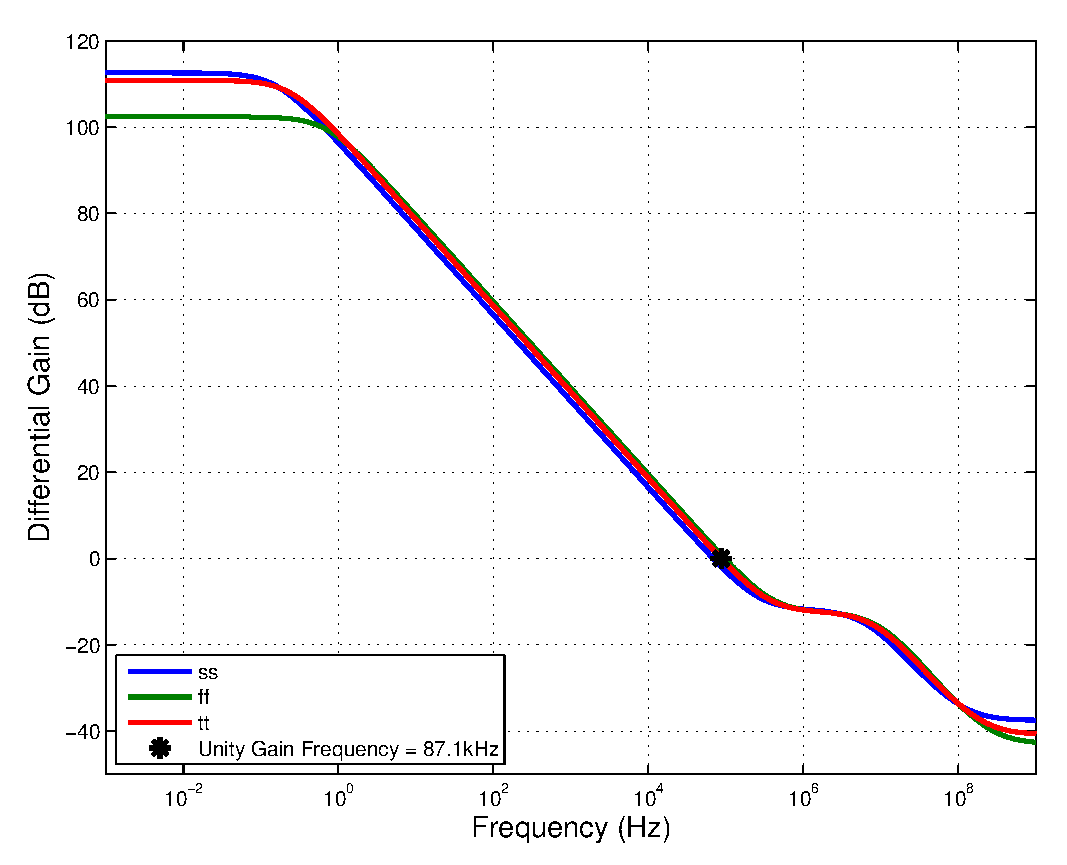
\includegraphics[width=4in]{Plots/open_dm_gain.eps}
\caption{The open loop differential gain magnitude response of the OTA.}
\label{fig:open_dm_gain}
\end{figure}


\begin{figure}
\centering
\includegraphics[width=4in]{Plots/open_dm_phase.eps}
\caption{The open loop differential gain phase response of the OTA.}
\label{fig:open_dm_phase}
\end{figure}

\subsection{Open Loop Common Frequency Mode Response}
In order for our OTA to be robust against common-mode noise, it is important for the common mode gain to remain very low across all frequencies. As can be seen in our plots for common mode gain (Figure \ref{fig:open_cm_gain}) and common mode phase (Figure \ref{fig:open_cm_phase}), common mode changes on the input have a very limited effect on the output.

\begin{figure}
\centering
\includegraphics[width=4in]{Plots/cmfb_gain.eps}
\caption{The open loop common mode gain magnitude response of the OTA.}
\label{fig:open_cm_gain}
\end{figure}

\begin{figure}
\centering
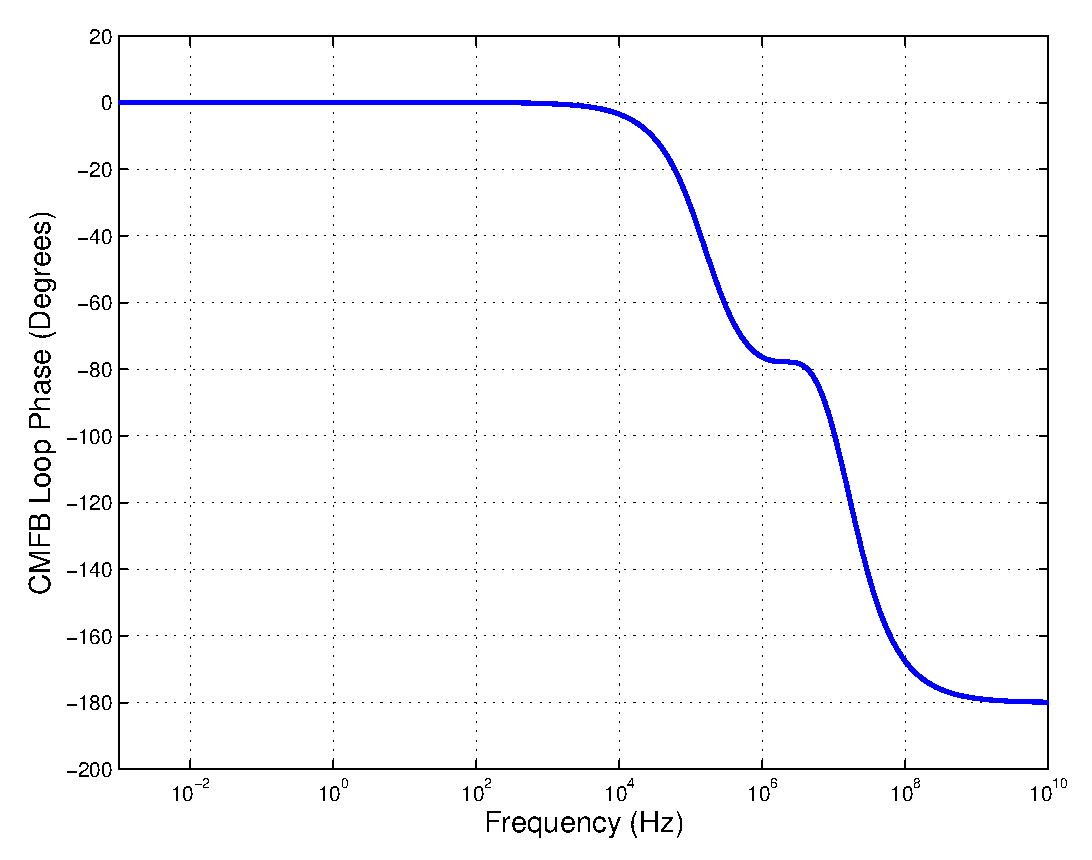
\includegraphics[width=4in]{Plots/cmfb_phase.eps}
\caption{The open loop common mode gain phase response of the OTA.}
\label{fig:open_cm_phase}
\end{figure}

\subsection{Common Mode Feedback Frequency Response}
Our goal in developing a common mode feedback (CMFB) network was to provide circuitry to hold our output node at $V_{CM}$. To ensure that our circuit was functioning as we intended, we broke our feedback loop at the input of the CMFB network and stimulated the circuit with a small signal source. We then measured the output of the CMFB circuit at the node that feeds back to our cascade branch. Our results can be seen in figures \ref{fig:open_cmfb_gain} and \ref{fig:open_cmfb_phase}.

\begin{figure}
\centering
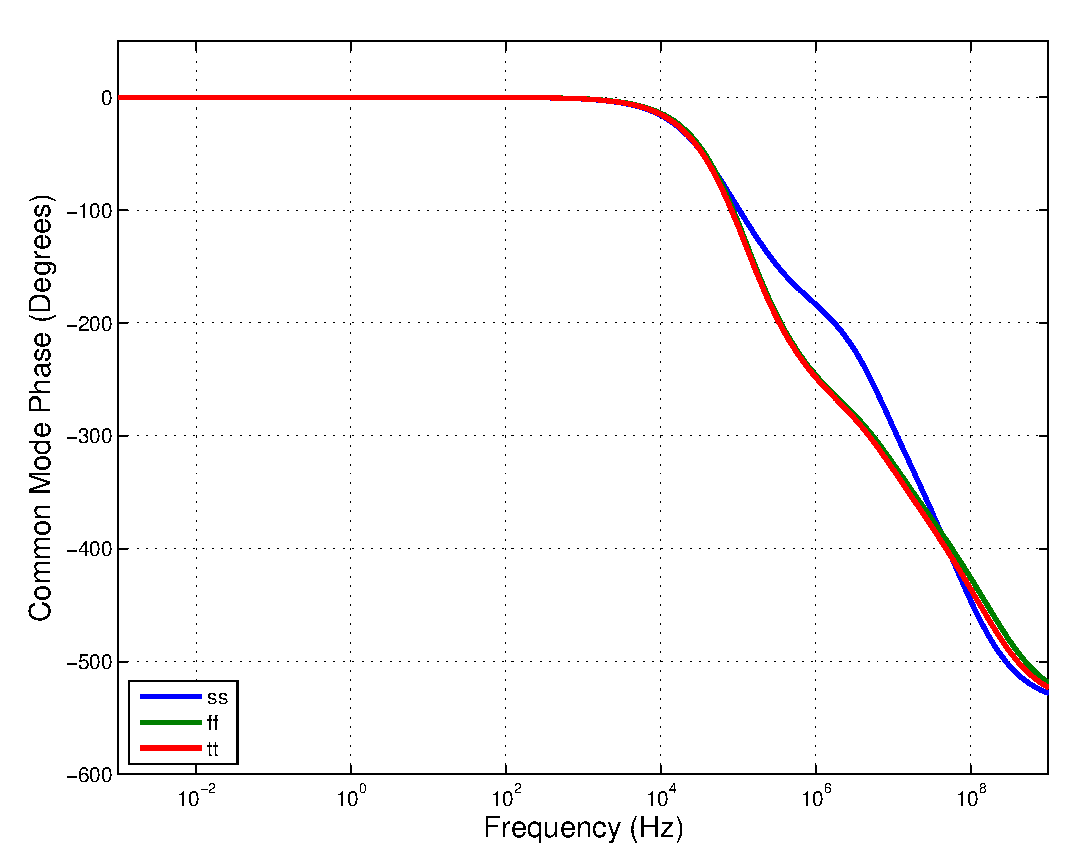
\includegraphics[width=4in]{Plots/open_cm_phase.eps}
\caption{The common mode feedback network gain phase response.}
\label{fig:open_cmfb_gain}
\end{figure}

\begin{figure}
\centering
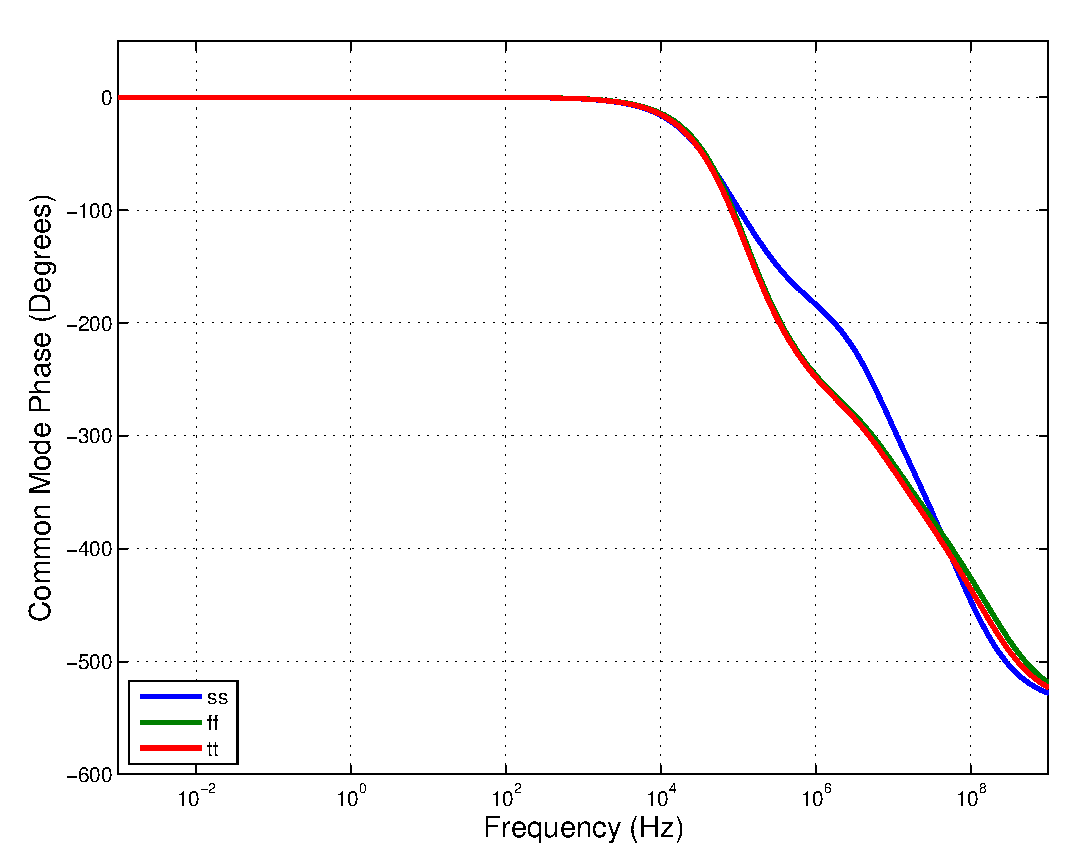
\includegraphics[width=4in]{Plots/open_cm_phase.eps}
\caption{The common mode feedback network gain magnitude response.}
\label{fig:open_cmfb_phase}
\end{figure}


\section{Closed Loop Amplifier Results}
After we verified that we had met our open loop OTA specifications, we replaced the ideal OTA in our system level design with our own OTA design to verify that we still met the system level specifications.

\subsection{Nyquist Rate Sinusoidal Transient Response}
The first test we ran on our system was a sine wave input at our full-scale amplitude and the Nyquist frequency. As can be seen in our plot (Figure \ref{fig:closed_sine}), our system samples the input at the end of the sample phase to be $0.35V$ ($V_{FS}$). Over the course of the hold phase, the output slews and then settles linearly to a value of $1.402V$. This is within our maximum error value (shown below) and shows that our circuit successfully handles a sine wave input. The maximum input referred error we can tolerate is

\begin{equation}
4*\frac{V_{LSB}}{2} = 5.4mV
\end{equation}

\begin{figure}
\centering
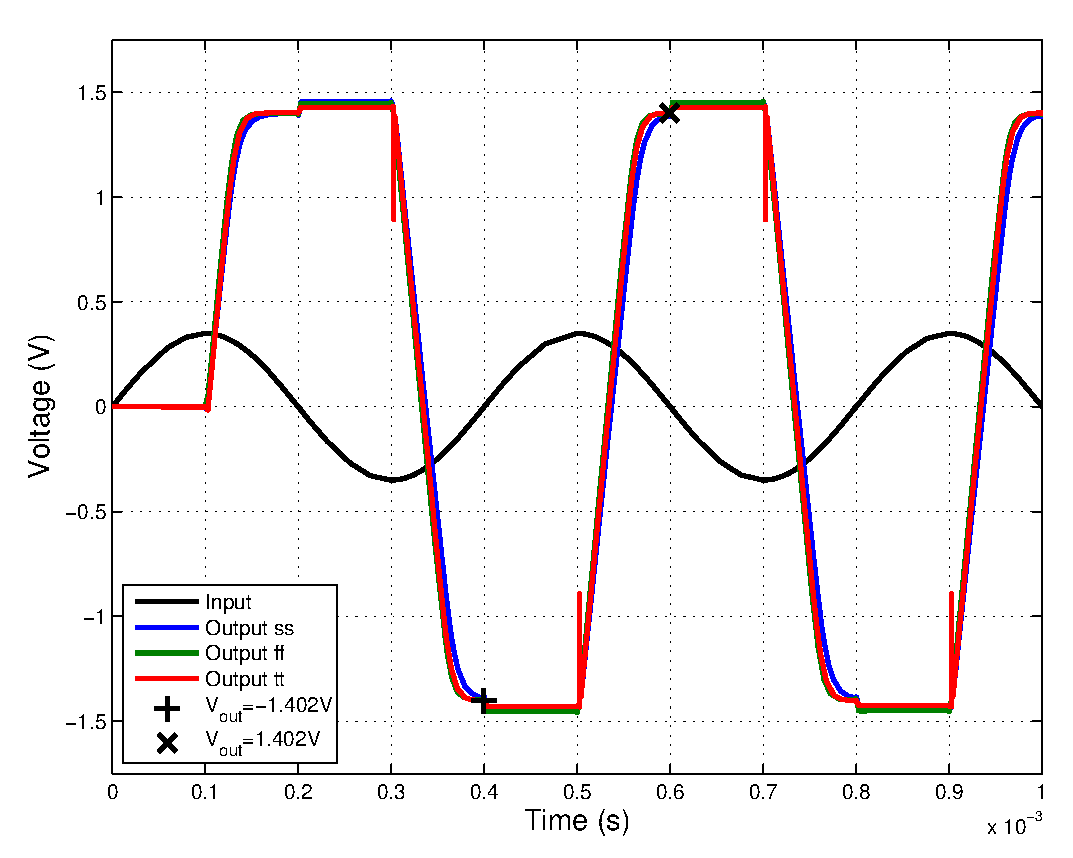
\includegraphics[width=4in]{Plots/closed_sine.eps}
\caption{The closed loop transient response to a full-scale amplitude sinusoid at the Nyquist frequency.}
\label{fig:closed_sine}
\end{figure}


\subsection{Small Step Transient Response}
The second test we performed on our closed loop system was a small step input. As can be seen in figure \ref{fig:closed_small_step}, our output shows a fast settling with little to no slewing. We provided an input step of $2mV$ and observed the output to settle to $8.012mV$ at the end of the hold phase. This is well within our spec for error so this test was successful.

\begin{figure}
\centering
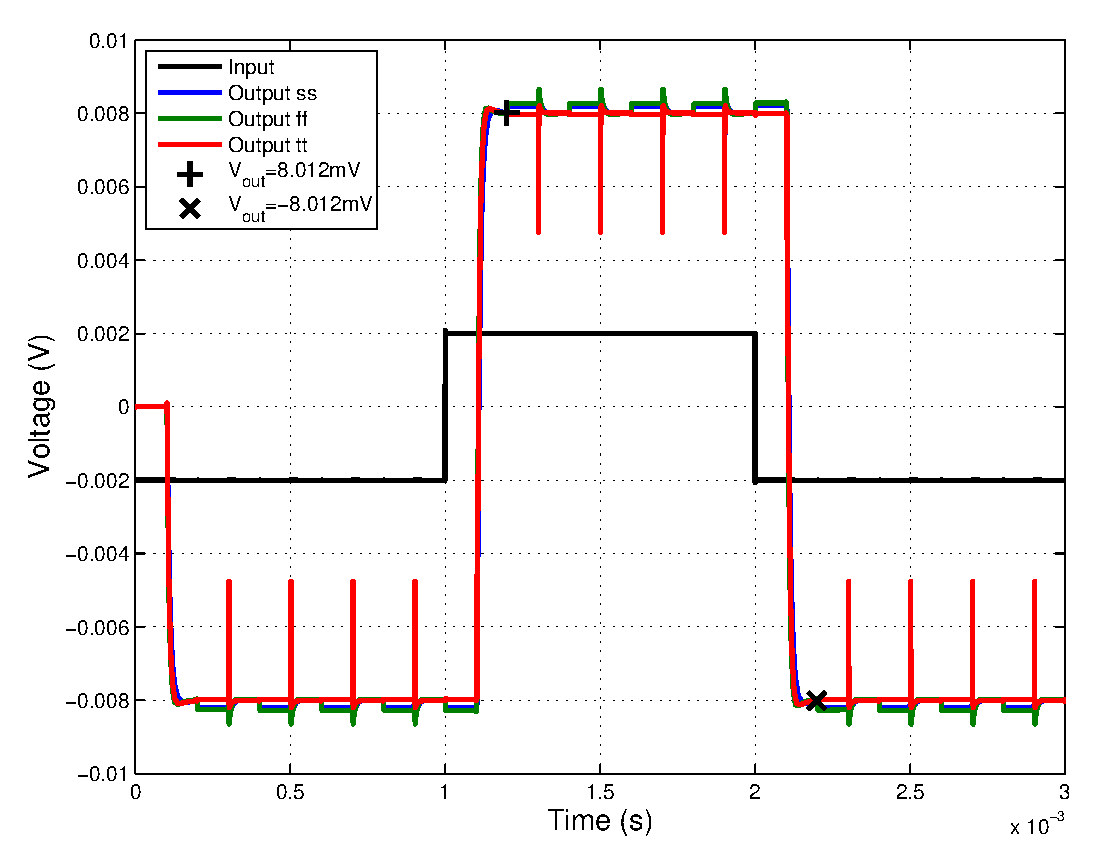
\includegraphics[width=4in]{Plots/closed_small_step.eps}
\caption{The closed loop transient response to a small amplitude step input.}
\label{fig:closed_small_step}
\end{figure}


\subsection{Full Scale Step Transient Response}
The third test we performed on our closed loop system was a step input at the full-scale voltage. The results of this test closely resembled those of the sine wave input. The reason for this is that the input is again sampled at the full-scale voltage and the output settles accordingly. This test was successful.

\begin{figure}
\centering
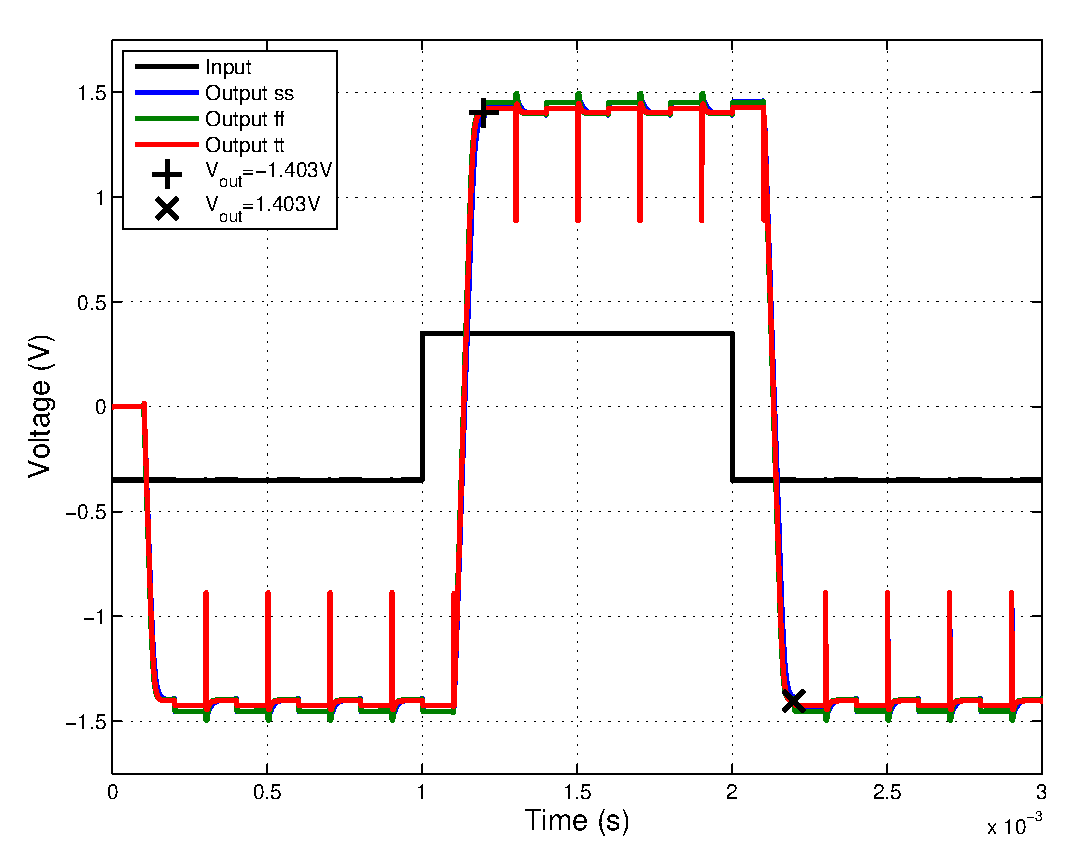
\includegraphics[width=4in]{Plots/closed_large_step.eps}
\caption{The closed loop transient response to a full-scale amplitude step input.}
\label{fig:closed_large_step}
\end{figure}

\subsection{Sawtooth Transient Response}
The fourth and final test we performed on our closed loop system was a sawtooth input at $f_s/20$. As can be seen from our plot in figure \ref{fig:closed_saw}, our system has no problem settling to the correct output for small changes in the input (along the ramp of the sawtooth). In addition, our output settles to the correct output in time after the edge of the sawtooth when the input drops from the full-scale voltage to the negative full-scale voltage.

\begin{figure}
\centering
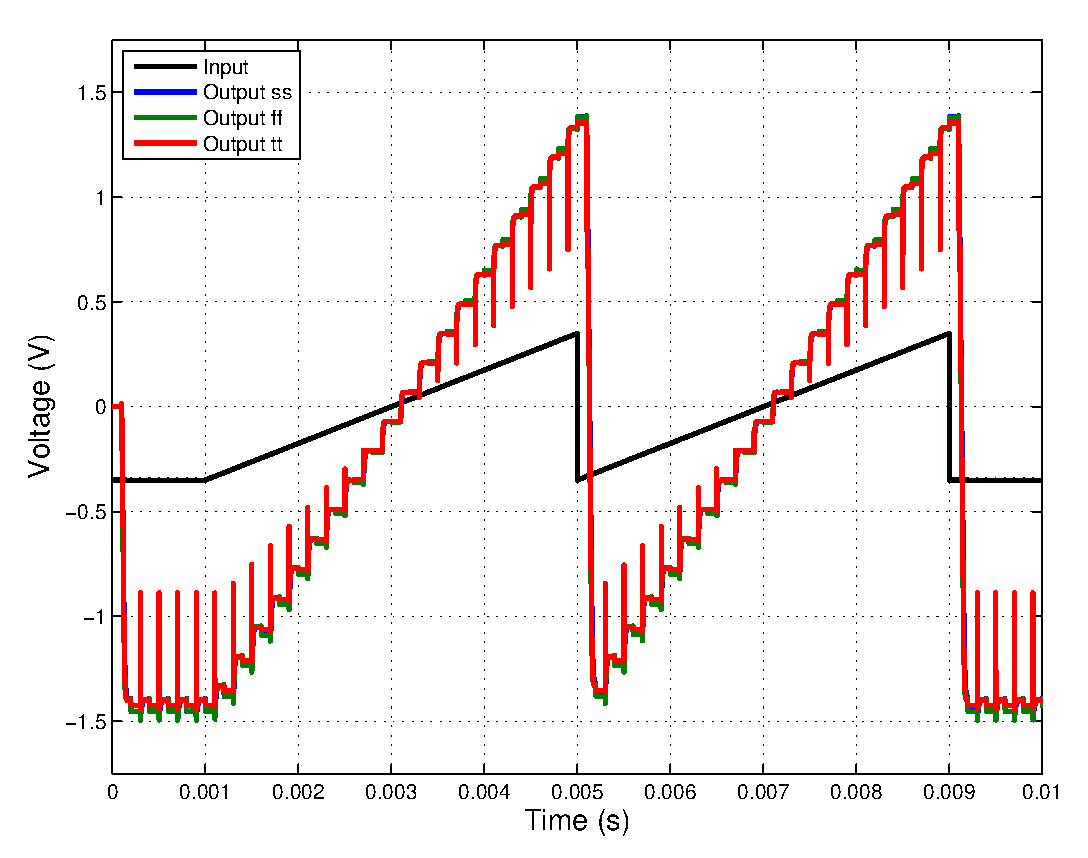
\includegraphics[width=4in]{Plots/closed_saw.eps}
\caption{The closed loop transient response to a full-scale amplitude sawtooth with a frequency of $\frac{f_s}{20}$.}
\label{fig:closed_saw}
\end{figure}

\subsection{Effective Number of Bits}

\subsection{Figure of Merit}
We calculated our figure of merit based on both the DC power consumption of our system as well as the average overall power of our system. Both values of power are shown in table \ref{tab:specs_results} and the FOM values are shown below.

\begin{equation}
FOM_{DC-POWER} = \frac{Power_{dc}}{2^{ENOB}f_s} = 150.3 fJ
\end{equation}

\begin{equation}
FOM_{TOTAL-POWER} = \frac{Power_{total}}{2^{ENOB}f_s} = 441.4 fJ
\end{equation}

\subsection{Area}
With the functionality of our system verified and its performance measured, we made an estimation of the area of our design. To measure the area of the transistors in the design, we used the below formula where $L_{diff} = 0.48 \mu m$ and $\alpha = 1.3$.

\begin{equation}
Area_{transistors} = W*(L+L_{diff})*\alpha = 55.50 pm^2
\end{equation}

To calculate the area of the capacitors in our circuit, we used the below formula across all of our capacitors where $C_{unit-area} = 1fF/\mu m^2$.

\begin{equation}
Area_{capacitors} = \sum{C/C_{unit-area}} = 3.00 nm^2
\end{equation}

Finally, to calculate the area of the resistors in our circuit, we used the below formula across all of the resistors in our design where $R_s = 10\Omega / \mu m^2$.

\begin{equation}
Area_{resistors} = \sum{R/R_s} = 8.00 \mu m^2
\end{equation}

Adding the above results for area, we came to a total area estimation as shown below.

\begin{equation}
Area_{total} = 8.0036 \mu m^2
\end{equation}

\section{Summary of Results}
As can be gathered from our numerical results, we successfully reached the goal we set out to accomplish. We designed a $10bit$, $5k sample/s$ amplifier for use in a $2.5bit/stage$ pipelined analog-to-digital converter which settles to an input referred error value less than $\frac{V_{LSB}}{2}$. In the process of designing this amplifier, we were able to maintain a very low value of total power consumption and as a result, a very respectable figure of merit. Thanks to a well thought out design process, we built and amplifier that not only meets its specs, but also maintains those specs over all PVT corners. If this design was put onto silicon and distributed to customers, we believe that it would prove to be robust enough to handle constant unpredictable use.

\begin{table}
\centering
\caption{Summary of Specifications and Results}
\label{tab:specs_results}
\begin{tabular}{|c|c|c|c|c|}
\hline Specification & Specification Value & FF Result & TT Result & SS Result\\ 
\hline Open Loop OTA DC Gain & $72.20 dB$ &$102.38 dB$&$110.86 dB$&$112.57 dB$\\ 
\hline Open Loop OTA Phase Margin & $60^o$ & $75.4^o$ & $75.2^o$ & $74.3^o$ \\ 
\hline Open Loop OTA Unity Gain Bandwidth & $44.10kHz$ & $96.93kHz$ & $87.34 kHz$ &  $68.83 kHz$ \\ 
\hline DC Power Consumption & -- & $747.90 nW$ & $769.50 nW$ & $803.16 nW$\\ 
\hline Overall Power Consumption & -- & -- & $2.26\mu W$ & --\\ 
\hline DC Figure of Merit & -- & -- & $150.3 fJ$ & --\\ 
\hline Overall Figure of Merit & -- & -- & $441.4 fJ$ & --\\ 
\hline Overall Area & -- & -- & $8.0036 \mu m^2$ & -- \\ 
\hline 
\end{tabular} 
\end{table}


\section{Possible Improvements}
While most of the specifications of our finished amplifier are impressive, one that needs optimization is the total area. Because we originally set out to meet a more stringent specification for gain, we were forced to utilize two $40\Omega$ resistors in the CMFB circuit. These two resistors account for the vast majority of the design's area. Because we ultimately were able to attain a gain far greater than the requirement, in future optimizations of the design we would focus on bringing the value (and hence size) of these resistors down to a more reasonable value. In addition, we believe that with redesign of the OTA, we can achieve a much lower power consumption and utilize much smaller compensation capacitors.

\section{Conclusion}
Through the design of this amplifier, we were able to attain a good deal of knowledge on new circuit techniques as well as design process. Unlike some of our previous designs, we spent a very long time developing our ideas on paper until we were satisfied that they would give us the results we were looking for. Thanks to this patience, once we put our theories into simulation, we were very pleased with the results. We were able to hit our spec after the first iteration of design and we spent most of the remaining design time optimizing for power and accuracy.
This project is quite appropriate for the class because it allows a broad range of students with different backgrounds to show interest. Because the design requires some knowledge of digital theory in addition to the heavy analog theory, a strong need for collaboration was instilled and led to a much more organic learning environment. 

% references section

% can use a bibliography generated by BibTeX as a .bbl file
% BibTeX documentation can be easily obtained at:
% http://www.ctan.org/tex-archive/biblio/bibtex/contrib/doc/
% The IEEEtran BibTeX style support page is at:
% http://www.michaelshell.org/tex/ieeetran/bibtex/
%\bibliographystyle{IEEEtran}
% argument is your BibTeX string definitions and bibliography database(s)
%\bibliography{IEEEabrv,../bib/paper}
%
% <OR> manually copy in the resultant .bbl file
% set second argument of \begin to the number of references
% (used to reserve space for the reference number labels box)
%%\begin{thebibliography}{1}
%%
%%\bibitem{sedrasmith}
%%A.~Sedra and K.~Smith, \emph{Microelectronic Circuits}, 6th~ed. \\ 
%%Oxford University Group, 2009. pgs. 711-716.  
%%\bibitem{LowGroupDelay}
%%Kim, J.; Buckwalter, J.F.; "Bandwidth Enhancement With Low Group-Delay Variation for a 40-Gb/s Transimpedance Amplifier," \emph{Circuits and Systems I: Regular Papers, IEEE Transactions on} , vol.57, no.8, pp.1964-1972, Aug. 2010.
%%
%%\end{thebibliography}

%\bibliographystyle{plain}
%\bibliography{AnalogProjectReferences}
\section{Seminar Responses: Joseph Meyer}
\subsection{Dr. Deepnarayan Gupta: Superconductor Electronics and Digital-RF Technology}
Dr. Gupta's seminar covered a vague interest of mine: combining superconductor and semiconductor electronics. Before this lecture, I wondered why these sorts of circuits taking advantage of superconductors' almost magical properties weren't more common. It seems that the main reason why these types of systems aren't more common are actually pretty obvious: you need to cool the systems down to 4K. More so than requiring a lot of power, the cooling systems consume a large amount of space, at least a couple of cubic feet. That sort of space requirements make these systems impractical in many scenarios.

Dr. Gupta said that biggest advantage of these systems is the high sensitivity. Indeed, I don't think thermal noise is going to be much of an issue at 4K. Dr. Gupta also mentioned that the primary limiting factors in these systems involved the analog to digital converters and the reliable packaging. The interconnects between modules must be able to handle data transfer at the high frequencies at which these circuits are operating.

I was especially intrigued as to why some the systems from HYPRES involved both high and low temperature superconductors. I asked Dr. Gupta this question and he responded back that having different stages of temperatures allowed for an easier heat load on the low temperature superconductors.


\subsection{Dr. Simone Gambini: More than Moore Comes of Age}
Dr. Gambini's lecture provided an interesting and different view about the future of devices. I've typically heard about whats the big, new thing that is going to REPLACE CMOS. Graphene, carbon nanotubes, and quantum electronics all come to mind. However, Dr. Gambini argued more that the future isn't what is going to replace CMOS, but what is going to work with it. Future microelectornic systems will have the ability to interface with many more new different technologies such as silicon photonics, sensors, MEMS devices, printed transistors and other semiconductor materials. Designers of the future must be able to cover larger different design spaces to create optimal systems. 

I found the ideas about circuits embedded into people that sent out information ``off body'' more than mildly interesting. Specifically, the fact that transmitter design in these systems was vastly more important than receiver design since the transmitter must do its work from within the body.

I was a little skeptical about the ideas and results on the study of the brain that was done. The assumption that any part of the channels of neurons in the brain act linearly seems to me to be overly optimistic. He was pretty upfront about the challenges associated with stimulating and measuring the brain at the same time. We might find that this is all but impossible.


\subsection{Dr. Junhua Shen: The Journey to High Speend and High Resolution SAR ADCs}
It is well know that there are immediate tradeoffs in converter design between speed, resolution and power. Dr. Shen showed ways in which to maximize the performance of an ADC by combining elements of various kinds. SAR ADCs are known for being accurate; but slow. The ADC that Dr. Shen presented got around some of the latency problems of a typical SAR ADC by determining the first 5 or so bits with a simpler and faster flash architecture. The inaccuracies and non-idealities of the flash were compensated by redundancies in the bits of the SAR part of the design. 

One theme for achieving better performance in design was to convert offset errors and mismatch into noise errors by implementing extra bits or an extra DAC which can be selected to be used. Having three DACs for use in the ADC caused problems when laying out the structure. Three of anything is harder to keep symmetric and even from a layout perspective than an even number of the same thing.

When asked, Dr. Shen said that disturbances caused by agressors and victims were the hardest problems faced through the design because of their unpredictability.

\section{Seminar Responses: Miles Sherman}
\subsection{Simone Gambini: More Than Moore Systems}
Dr. Gambini gave an informative and interesting perspective on his work and the industry as a whole. While I was previously aware of a good amount of "More Than Moore" work being done, getting a feel for some specific projects was helpful for my understanding. The one aspect of this seminar that stuck with me was the fact that the noise associated with actually stimulating brain activity is actually larger than the brain's signal poses an interesting problem and a demand for a solution. There is definitely a lot of room for major development in this field.

\subsection{Adad Abidi: Armstrong's Circuits \& The Worldwide Spread of Radio}
Of the three seminars I attended this semester, I would say this one was the most interesting for me. Dr. Abidi presented the work of Edwin Armstrong in a very specific way so as to motivate a connection between the work of the 1920's and the analog design of today. Armstrong's circuits played a major role in influencing the way we communicate today and it is	clear when his fundamental designs are found in the large systems of analog communication chips in modern day devices. Armstrong's main focus in his work seems to be resourcefulness since vacuum tubes were so expensive. Modern day engineers can learn a lot from his work. Even though transistors are a commodity now, there is always optimization to be done.

\subsection{Shanthi Pavan: Continuous-Time Delta Sigma Data Converters}
This was the final lecture I attended and I probably had the most trouble following this one due to its more in depth technical discussion of a new topic for me. Dr. Pavan discussed new techniques for the elimination of clock-jitter and non-linearities in delta sigma converters. While I could not follow his exact method of innovation, I was certainly able to learn a good amount about the operation of delta sigma converters. These systems operate by oversampling the input at sampling rates much higher than those at the final output of the system. By doing this, the system can then modulate the noise and push it to higher frequencies than those of interest. The signal is then re-sampled and outputted.

\end{document}